\documentclass[border=2pt]{standalone}
\usepackage{times}
\usepackage{amsmath,amssymb}
\usepackage{tikz}
\usetikzlibrary{arrows.meta,calc,positioning}
\begin{document}
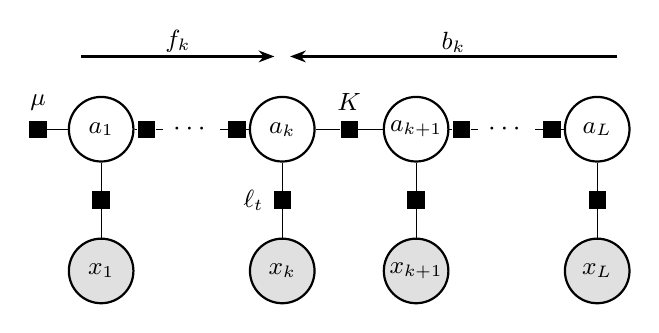
\begin{tikzpicture}[
    var/.style={circle,draw,thick,minimum size=8.2mm,inner sep=0pt,font=\small},
    obs/.style={circle,draw,thick,fill=black!12,minimum size=8.2mm,inner sep=0pt,font=\small},
    fac/.style={rectangle,fill=black,minimum size=2.2mm,inner sep=0pt},
    lab/.style={font=\small,inner sep=1pt},
    msg/.style={-{Stealth[length=2mm]},thick}]
  \node[var] (a1) at (0,0) {$a_1$};
  \node (d1) at (1.15,0) {$\cdots$};
  \node[var] (ak) at (2.3,0) {$a_k$};
  \node[var] (ak1) at (4.0,0) {$a_{k+1}$};
  \node (d2) at (5.15,0) {$\cdots$};
  \node[var] (aL) at (6.3,0) {$a_L$};
  \node[fac] (m0) at (-0.8,0) {};
  \draw (m0) -- (a1);
  \node[lab,above=0.8mm of m0] {$\mu$};
  \foreach \u/\v/\n in {a1/d1/ka,d1/ak/kb,ak/ak1/kc,ak1/d2/kd,d2/aL/ke} {
    \node[fac] (\n) at ($(\u)!0.5!(\v)$) {};
    \draw (\u) -- (\n) -- (\v);
  }
  \node[lab,above=0.8mm of kc] {$K$};
  \foreach \i/\n in {a1/1,ak/k,ak1/{k+1},aL/L} {
    \node[fac] (o\i) at ($(\i)+(0,-0.9)$) {};
    \node[obs] (x\i) at ($(\i)+(0,-1.8)$) {$x_{\n}$};
    \draw (\i) -- (o\i) -- (x\i);
  }
  \node[lab,left=0.8mm of oak] {$\ell_t$};
  \draw[msg] ($(a1.north)+(-0.25,0.5)$) -- node[lab,above]{$f_k$} ($(ak.north)+(-0.1,0.5)$);
  \draw[msg] ($(aL.north)+(0.25,0.5)$) -- node[lab,above]{$b_k$} ($(ak.north)+(0.1,0.5)$);
\end{tikzpicture}
\end{document}
